%% LyX 1.5.3 created this file.  For more info, see http://www.lyx.org/.
%% Do not edit unless you really know what you are doing.

\documentclass[12pt,english,a4paper]{article}
\renewcommand{\familydefault}{\rmdefault}
\usepackage[T1]{fontenc}
\usepackage[latin9]{inputenc}
\usepackage{geometry}
\geometry{verbose,letterpaper,tmargin=2.5cm,bmargin=2.5cm,lmargin=2.5cm,rmargin=2.5cm}

\setcounter{secnumdepth}{-1}
\setcounter{tocdepth}{-1}

\usepackage{booktabs}
\usepackage{textcomp}
\usepackage{amsmath}
\usepackage{graphicx}
\usepackage[authoryear]{natbib}
\usepackage{setspace}

\doublespacing
\makeatletter

%%%%%%%%%%%%%%%%%%%%%%%%%%%%%% LyX specific LaTeX commands.
%% Because html converters don't know tabularnewline
\providecommand{\tabularnewline}{\\}
%% A simple dot to overcome graphicx limitations
\newcommand{\lyxdot}{.}


%%%%%%%%%%%%%%%%%%%%%%%%%%%%%% User specified LaTeX commands.
 

\usepackage{amsfonts}


% \usepackage{biocon}
% 
% \newplant{potr}{Populus tremuloides}
% \newplant{tsca}{Tsuga canadensis}
% \newfungus{}
% \newfungus{}
% \newfungus{}
% \newfungus{}
% \newfungus{}
% \newfungus{}
% \newfungus{}
% \newfungus{}
% \newfungus{}
% \newfungus{}
% \newfungus{}
% \newfungus{}
% \newfungus{}
% \newfungus{}
% \newfungus{}
% \newfungus{}

% Title Page
\author{David LeBauer}
\date{\today}

\AtBeginDocument{
  \def\labelitemii{\(\circ\)}
  \def\labelitemiii{\(\cdot\)}
}

\usepackage{babel}
\makeatother

\begin{document}

\title{Fungal Diversity and Decomposition Microcosm Study}

\maketitle

\section{Abstract}

\section{Introduction}

 As humans extinguish species, it is useful to know how these losses affect ecosystem functions \citep{chapin2000ccb,ehrlich2008wdb}.
 The link between biodiversity and ecosystem function has been widely observed, and suggests that local and global declines in species diversity can reduce the ecosystem services upon which humans depend \citep{hooper2005ebe}.
 Models predict an asymptotic relationship between plant species number and plant biomass is common \citep{tilman1997pde}.
 Among twenty diversity manipulation experiments, nineteen exhibited significant positive relationships between diversity and function \citep{schwartz2000lbe}.
 Previous studies show that species number and identity affect ecosystem functions at many trophic levels \citep{schwartz2000lbe,cardinale2006ebf}.
 Frequently the number of species positively affects function, in addition, the identity of component species also affects the relationship between biodiversity and ecosystem function \cite{cardinale2006ebf}.
 Because of these relationships, human impacts that reduce species diversity or alter the composition of microbial communities can influence ecosystem function.
 


 In addition to above effects on biomass, a positive effect of decomposer diversity on decomposition is also frequently observed, although the effect can also be neutral or negative \citep{loreau2001mdp,jiang2008ins}.
 Previous studies frequently link biodiversity to positive effects on biomass production within all trophic levels \citep{cardinale2006ebf}.
 In contrast to the biomass of the decomposer community, the rate of decomposition responds less consistently to diversity \citep{jiang2008ins}.
 Decomposition often increases \citep{tiunov2005fir,setala2004dro}, but frequently does not respond \citep{hedlund2000tis,dang2005mvp} and sometimes declines \citep{janzen1995clc,toljander2006eff} with increasing decomposer diversity.

 The primary biotic mechanism used to explain a positive effect of species diversity on function is niche partitioning.
 Niche partitioning results in increased total resource use because variation in resource acquisition traits among species increases the diversity of resources that can be utilized  \citep{tilman1997pde}.
 Among decomposers, niche partitioning is expected to increase the efficiency of nutrient cycling and carbon mineralization \citep{loreau2001mdp}.
 Two decomposers that utilize different substrates should increase total substrate utilization when the two species are grown together compared to either species in monoculture.
 The partitioning of resources is associated with fungi that specialize on distinct substrates.
 Unlike niche partitioning, the sampling effect results from the increased probability of sampling a high yield species when number of species sampled increases \citep{loreau2001psc}.
 
 Facilitative interactions also result in a positive link between diversity and function; this is when the presence of one species improves the growth of another species. 
 For example, plant litter is a primarily a matrix of cellulose interlinked with and stabilized by lignin, and the decomposition of lignin can increase the amount of cellulose that is available to cellulose-degrading fungi.
 In this way, the presence of two species enables decomposition of a larger proportion of the total litter.
 Because fungi vary in their ability to produce the enzyme that degrade lignin and cellulose \citep{trigiano1979ees,novotny2004lfb,hatakka1994lme,baldrian2008dcb}, fungal species that target different substrates within this matrix can decompose a complex substrate more rapidly when grown as a pair than when grown individually.
 For this reason, specificity among individual species is predicted to link increased decomposer biodiversity to increased overall recycling efficiency of organic compounds by a decomposer community \citep{loreau2001mdp}.
 This interaction can result in the strong positive effect observed when cellulose degrading ascomycetes and lignin degrading basidiomycetes alternate growth during decomposition \citep{fog1988ean}.
 Similarly, decomposition of cellulose by \emph{Chaetomium thermophile} increases when a non-cellulolytic fungus, \emph{Thermomyces lanuginosusa} was present \citep{deacon1985dfp}.
 By demonstrating a stronger relationship between species number and decomposition of simple compared to complex substrates, Tiunov and Scheu (2005)\nocite{tiunov2005fir} provide further support for an important role of facilitative interactions in decomposition.

 On the other hand, not all ecosystem functions are expected to increase with species number, and neutral or negative responses are expected in particular for functions other than biomass production \citep{jiang2008ins}.
 For example, niche partitioning implies that resource availability will decline as resources are more fully exploited under the same conditions that result in a positive plant diversity -  biomass BEF relationship \citep{hooper1998epc,cardinale2006ebf}.
 In general, ecosystem functions other than biomass should be expected to yield either positive, neutral, or negative BEF relationships \citep{jiang2008ins}.
 Furthermore, models predict that the efficiency of decomposition can only decline or not change as the diversity of plants and organic compounds increases \citep{loreau2001mdp}.
 This occurs because substrate diversity increases available niche space but inhibits any individual species from becoming competitively dominant. 
  Negative interactions can also occur when a species produces antagonistic compounds, this trait not only inhibits the growth of other organisms, it diverts resources from biomass production \citep{jiang2008ins}.

% On the other hand, increasing the diversity of substrates 
%%%Paragraph: elaborate on sp - ecosystem fn link, mechanisms
%%%Identify gap in our knowledge that the present study will address

 The contribution of individual decomposer species to decomposition and enzyme production is not tractable in the same way that the contribution of individual plant species to biomass is.
 For this reason, it is not possible to empirically determine the relative contributions of niche partitioning and the selection effect to BEF relationships among decomposers and decomposition with the same equations used for plants \citep{loreau2001psc,fox2005ise}.
 Tinuov and Scheu's (2005) \nocite{tiunov2005fir} observation that the positive effect of species on decomposition is significantly stronger on cellulose compared to diverse soil carbon compounds substrates indicates that facilitative interactions are more important than resource partitioning.
 This observation is consistent with Loreau's (2001) model prediction that substrate diversity can inhibit decomposition.
 However, I am aware of no studies that directly evaluate the effects of species diversity on resource use and partitioning among decomposers on a complex substrate.
 To better understand the role of resource partitioning in the relationship between diversity and decomposition, the present study investigated the response of decomposition and the activity of enzymes that target two distinct substrates: lignin and cellulose.
  
 Because substrate use and enzyme production varies among species of fungi \citep{trigiano1979ees,hatakka1994lme,baldrian2008dcb,allison2009lln}, I hypothesized that litter decomposition rate would increase with the number of species in laboratory fungal communities.
 Furthermore, I predicted that the activities of lignin and cellulose-degrading enzymes would increase with species number.
 To evaluate relationships among the diversity of fungal communities, enzyme activity, and decomposition, I isolated functionally diverse fungi and conducted a laboratory microcosm experiment in which I manipulated species number.

 %Setala and McLean concluded that niche partitioning was responsible for the observed increase in decomposition in high relative to low diversity fungal communities \citepp{setala2004dro}.

% By contrast, the production of PPO is a trait that is primarily found among white-rot Basidiomycetes, although  Ascomycetes and Basidiomycetes \citepp{baldrian2006flo}, they are often .

\section{Methods}


\subsection{Isolation of Fungi}


 All fungi were collected near Delta Junction, Alaska 63$^{\circ}$55'N, 145$^{\circ}$44'W in the region described in detail by Treseder et. al. (2004)\nocite{treseder2004raf}.
 These boreal forests are diverse in age (time since fire) and included mature black Spruce (\textit{Picea mariana}) stands as well thin stands of Aspen (\textit{Populus tremuloides}) recovering from a recent fire and interspersed with standing dead Spruce.
 I collected fungal fruitbodies and colonized substrate from coarse litter including Spruce boles and roots remaining from previous fires, as well as forest floor litter, and soil from the O-horizon. %I also included the ubiquitous and abundant white-rot fungus \textit{Trametes versicolor} collected from a wood pile at the Silver Fox Roadhouse addition, I collected including Black Spruce boles to mature stands of \textit{P. mariana} 
 
 I cultured fungal isolates directly from mushroom tissue, litter, and wood using malt yeast agar (MYA) ammended with selective antibiotics.
 The primary selective media was malt yeast agar (MYA: 5 g malt extract, 5 g yeast extract, 20 g agar per liter) with selective biocides {6 mg 2-phenyl-phenol and 8 mg benomyl} added to inhibit bacteria and lower fungi \citep{carey1989smi}.
 In addition, I selected two previously cultured isolates previously cultured from soil at the control burn site \citep{treseder2004raf}, \textit{Pennicilium} sp. and \textit{Mortierella} sp., which account for 0.2-1.0\% and 0.4-2.4\% of the fungal community, respectively \citep{allison2009lln}.
 These two isolates were isolated on minimal nutrient agar containing 500 mg KH$_2$PO$_4$, 150 mg MgSO$_4$·7H$_2$O, 50 mg CaCl$_2$·2H$_2$O, 25 mg NaCl, 20 mg ferric EDTA, 0.1 $\mu$g thiamine HCl, 12 g agar, 130 $\mu$g streptomycin, and 10 mg chlortetracycline and either 250 mg (NH4)3PO4, 3 g malt extract, and 10 g glucose (\textit{Pennicilium} sp.) or 1 mg malt extract, 1 g bovine serum albumin, and 10 g tannic acid (\textit{Mortierella} sp.) \citep{allison2009lln}.
 I chose the sixteen fungi from over one hundred isolates to represent the the overall diversity of morphology, growth rate, and phylogeny observed among the initial pool of isolates, and to be consistent with the fungal taxa found in these forests \citep{allison2007nfr}.
 Among the sixteen isolates, growth rate on MYA ranged from 0.05 to 0.9 cm d$^{-1}$, and I used both macro and microscopic morphological characters including fruiting structure, clamp connections, and the  shape, texture, and color of the culture to select a subsample of fungi representative of the \textit{in situ} community.

 Using morphological characters in combination with 18S and ITS sequences of fungal rRNA genes (allison2008mas), we were able to identify some isolates to species and others to a broad taxonomic group.
 I extracted DNA from isolates growing on MYA using the Mo Bio Ultra Clean Plant DNA kit (Mo Bio Laboratories, Carlsbad, CA, USA), used PCR to amplify the DNA which was then sent to Agencourt Bioscience Corporation (Beverly, MA, USA) for sequencing.
 Using BLAST \citep{mcginnis2004bcp}, we matched 18S and ITS regions separately with GenBank accessions \citep{benson2007g}.
 The sixteen isolates included eleven Basidiomycetes and five frequently found non-basidiomycete fungi (Table \cite{tab:IsolateTable}).
 
\subsection{Experimental Design}

 I randomly assigned the sixteen isolates to treatments of one, two, four, or eight species; each species appeared with equal frequency at each treatment level.
 In the present study, the experimental unit of replication was a specific combination of species, and there was no true replication of any specific species mixture.
 The substrate was Aspen litter that had decomposed for twelve months in the field.
 This litter was collected from a 15-year old Aspen forest near Delta Junction, air dried, placed in 1-mm mesh nylon bags, affixed to the soil surface in the 80-year old site (control-burn) site in September 2005 and collected in September 2006.
 After collection of the litter, I dried it overnight at 60$^{circ}$C, ground it for sixty seconds in a coffee-millinto a coarse powder ($<$0.5 mm grains), and then exposed the litter to a sterilizing $\gamma$-irradiation of 2.5-3.0 Mrad in a self-shielded gamma irradiator with a CS-137 source (Shepherd and Associates, Mark I).

\subsection{Microcosms}
 For microcosms, I used 40 mL glass vials with rubber septa (No.SB36-0040, I-Chem).
 To maintain aeration and provide structure for the litter, I added 1.00 g of 30-60 grit sand to each of the vials, and then autoclaved the sand and the tube at 120$^{\circ}$C for 40 minutes.
 In a laminar flow hood, I transferred approximately 50 mg of sterile Aspen litter into each microcosm and recorded the mass of litter added.
 I created a liquid innoculum by homogenizing fungi growing on agar in a liquid growth medium. 
 I transferred a 125 $mm^3$ cube of an individual isolate growing on MEA to a 1.5 ml eppendorf tube, and recorded the mass of the cube.
 I then homogenized the cube with 0.5 mL growth medium in a 1.5 ml eppendorf tube using a mortar and pestil.
 The growth medium was a solution of 500 mg KH$_2$PO$_4$, 150 mg MgSO$_4\cdot$7H$_2$O, 50 mg CaCl$_2\cdot$2H$_2$O, 20 mg ferric EDTA and 0.1 $\mu$g thiamine HCl per liter \citep{allison2009lln}.
 After homogenizing the sample, I diluted 0.5 mL of the homogenate in approximately 14.5 mL of the growth medium, adjusting this volume for the initial mass of the cube so that each of the sixteen innocula had equal concentrations of the initial MYA culture.
 For each of the 176 species combinations, I mixed 1, 0.5. 0.25. or 0.125 ml of this liquid inoculum from the 1, 2, 4, or 8 component species in eppendorf tubes for a total volume of 1 mL, of which 0.6 mL was transferred to a microcosm tube to inoculate the litter.

\subsection{Decomposition rates}
 I sampled CO$_2$ concentration in microcosms at seven time points (6, 9, 15, 25, 45, 76, and 111 days).
 At each time point, I used a syringe to remove 10 ml of gas from the headspace, which I then injected into an EGM-4 infrared gas analyzer (PP Systems, Amesbury, MA) to analyze CO$_2$ concentration.
 After sampling, I removed caps under a sterile laminar flow hood to allow headspace to equilibrate with the ambient air for at least 5 min.
 I calculated total decomposition as the CO$_2$-C that accumulated between replacing the cap and the next sampling time.
 Total CO$_2$ released was divided by the initial mass of the litter in each vial, and I report total decomposition for the 111 day study in units of mg CO$_2$-C respired per g litter at the beginning of the experiment.

\subsection{Enzyme Activities}
%  Lignin and cellulose account for most of the carbon flux into terrestrial ecosystems, including leaf litter. 
  At the end of the 111 day study, I used colorometric assays  \citep{allison2006aee} to determine the activities of the cellulose degrading enzyme $\beta$-glucosidase (BG) and the lignin degrading enzyme polyphenol oxidase (PPO).
 First I added 10 ml of 50 mM pH 5.0 acetate buffer to each microcosm, then I vigorously swrilled the vials on a culture rotating machine at 90 rpm for one hour to create a homogenized slurry of buffer, litter, sand, and fungi.
 For each microcosm, I added 50 $\mu$L of this homogenate to 150 $\mu$L of a substrate solution in fourteen wells of a 96 well plate.
 The substrates used were 5mM $p$-nitrophenyl-$\beta$-glucopyranosidase to assay BG activity and 50 mM pyrogallol, 50 mM EDTA to assay PPO activity, in 5.0 pH acetate buffer.

 Each 96 well plate included seven analytical replicates for each of six microcosms. 
 In addition, I ran seven controls (homogenate plus buffer instead of substrate) for each microcosm to correct for absorbance of the homogenate.
 To correct for absorbance of the substrate, on each plate I ran six replicate controls for substrate without homogenate.
 After combining homogenate and substrate, the reactions incubated at 20$^{\circ}$C for 2-4 hours on a rotary shaker that was set just slow enough to prevent the sample from shaking out of the wells.
 At the end of the BG assay, I added 5 $\mu$L of 1 M NaOH to terminate the reaction and develop color from the pNp products.
 I used absorbance at 405 nm to calculate  the amount of pNp produced (for BG) or pyrogallol consumed (for PPO) from empirically determined extinction coefficients for each substrate.
 Enzyme activities are expressed in units of $\mu$mol substrate formed (for BG) or comsumed (PPO) per milligram of litter per hour $g^{-1}mg^{-1}h^{-1}$.
 
% \paragraph{Response Metrics} To parametarize the functional response, we will quantify growth rate (B) and time of maximum growth (M) in each microcosm. To do this, we will fit a generalized logistic growth curve to total CO$_2$ efflux (as functional response) such that, $$ \sum{CO_2} = A + \frac{C}{(1+T exp{-B(x-M)})^{1/T}} $$
% where A and C are the lower and uppper asymptopes; M is time of max growth rate, B is growth rate, T is ?.


\subsection{Data Analysis}
%for each test, describe which results would support / which would lead me to reject my hypothesis
% specify independent and dependent variable(s) for each test
%order results to match order of statistical tests in methods section
 To test the effect of species number on respiration and enzyme activity, I conducted a series of regressions with the natural species number as the independent variable and CO$_2$ respiration, BG activity, or PPO activity as the dependent variable.
 I evaluated both linear and log-linear regressions, and present results from the the model that explainined most of the variation \citep{setala2004dro}.
 A significantly positive slope would support my hypotheses.
 Next, I conducted analysis of variance (ANOVA) with 16 independent variables indicating the presence or absence of each of the sixteen isolates, and with CO$_2$ respiration, BG activity, or PPO activity as the dependent variable.
 If individual species affected decomposition or enzyme activity, I would conclude that species identity affects function.
 Unlike investigations of plant diversity effects on biomass, I could not quantitatively assess the relative importance of selection and complimentarity.
 This is because the equations that are used require observation of the contribution of individual species within a mixture to the response of interest, in this case CO$_2$ respiration, BG activity, and PPO activity \citep{loreau2001psc}.
 Finally, I used Pearson's correlation coefficient to test for correlations between BG or PPO activity and CO$_2$ respiration.
 A significant correlation would support my hypothesis that enzyme activity is an important control on decomposition.
 I omitted CO$_2$ and enzyme data from two leaky microcosms and enzyme data from a tray of twenty-four tubes that was misplaced prior to enzyme analysis; these excluded microcosms evenly distributed across treatments.
 Because the dependent variables CO$_2$ respiration, BG activity, and PPO activity did not meet the assumptions of the models applied, these variables were rank transformed.
 All analyses were performed using the \textit{lm} function in R \citep{rcore}. 

\section{Results}
 Total CO$_2$ released increased as a log-linear function of species diversity ($P=0.003$; $r^{2}=0.05$)(Fig. \ref{fig:obs.bg.v.spdiv}), as did BG activity ($P<0.001$; $r^{2}=0.16$).
 The increase in CO$_2$ released and BG activity was most rapid at lower levels of diversity, but was still increasing with species number at the maximum level of eight species in this experiment. In contrast, PPO activity did not significantly increase as a function of species number.
 
 Decomposition rate was not significantly affected by the presence of any single species (Fig. \ref{fig:sp.presence.absence}). 
 However, BG activity was significantly higher in microcosms that contained one of three isolates: \emph{Trametes versicolor} ($P=0.034$), \emph{Flammulina populicola} ($P=0.014$), or the unidentified Ascomycete ($P<0.0001$).
 Moreover, the presence of the unidentified Ascomycete had a marginally significant and negative effect on PPO ($P=0.051$).
 Emissions of CO$_2$ were marginally significantly correlated with BG activity ($P=0.07$; $r^{2}=0.014$), but not PPO activity  ($P=0.6$; $r^{2}=0.005$).

\section{Discussion}

%P1: the story
 Total CO$_2$ released from Aspen litter increased as a log-linear function of the number of species added to the microcosm  (Fig. \ref{fig:obs.bg.v.spdiv}).
 This response supports our hypothesis that the number of species present has a positive impact on decomposition. 
 Similarly, the log-linear increase in BG activity with species number supports my second hypothesis, and provides a possible mechanism for the increase in decomposition rate.
 From these results, I conclude that species diversity is important to both decomposition and BG activity, but there is no link between diversity and PPO activity.
 Although species diversity has similar effects on CO$_2$ release and BG activity, the positive correlation between BG and CO$_2$ was low and only marginally signficant.
 Therefore, support for a causal link between BG activity and decomposition is weak.

%P2:
 % how relates to what other people have done?
 % Two approaches to the study of diversity effects on funciton are:  removal from a native community and assemblage of isolates.
 %Hedlund and Sjogren Ohrn 2000 did not see 
    % contrast with elimination studies
% dilution/fumigation

 Positive relationships between the number of fungal species and the rate of decomposition have been previously demonstrated in experimental microcosms \citep{setala2004dro,robinson1993ncd,tiunov2005fir}.
 Among fifteen studies of decomposer species diversity effects on decomposition (measured as CO$_2$ release, O$_2$ uptake, or litter mass loss), nine report postive relationships \citep{jiang2008ins}.
 Similar to the present study, Setala and McLean \nocite{setala2004dro} report a log-linear response of CO$_2$ release to species number, indicating that the largest effects of species number occur at lower levels of diversity.
 To test the importance of facilitation and complimentarity, Tiunov and Scheu (2005) \nocite{tiunov2005fir} compared the effect of species number on decomposition of cellulose filters to the effect of species number on decomposition of soil organic matter. 
 They found that respiration of cellulose increased five fold, in direct proportion to the number (one through five) of species present. 
 By contrast, respiration of carbon from soil increased less than 20\% across the gradient of species number \citep{tiunov2005fir}.
 Their finding indicates that the increased respiration by diverse communities results from interspecific facilitation rather than resource partitioning, and supports Loreau's  model \citep{loreau2001mdp}.
 However, these previous studies provide no insight into resource partitioning on a complex litter substrate.   

% However, the opposite response also occurs.
% For example, Toljander et al. (2006) \nocite{toljander2006eff} observe reduced decomposition rates with increasing species diversity.
% In another study, decomposition is higher with one species of fungus on sterilized straw compared to multiple species of fungi \citep{janzen1995clc}.
% Decomposition of litter in a pine forest was greater when litter was pre-inoculated with a single fungal isolate prior to being decomposed by native microflora in the field compared to litter that was not pre-inoculated \citep{cox2001efi}.
% In that study, Cox et al (2001) find an effect on litter chemistry but not on total decomposition when the species used in pre-inoculation was a lignin versus a cellulose degrading fungus.

%%%%unique additions of present study
 In the present study, I evaluate the effect of fungal species diversity on the activity of extracellular enzymes involved in decomposition.
 Extracellular enzymes have been identified as primary controls on decomposition of organic matter \citep{sinsabaugh1994rae}.
 If enzyme activities serve as proxy for substrate utilization, a positive effect of diversity on decomposition would be accompanied by an increase in the activity of enzymes that degrade the respired substrate.
 The increase in activity of the cellulose degrading enzyme BG with species number in the present study supports increased utilization of cellulose at higher levels of species diversity.
 This response is consistent with the facilitative interactions observed on cellulose \citep{tiunov2005fir}.
 
%P3:
   %diversity w/changes related to global change
 Most microbial communities are sensitive to components of global change including warming, increased CO$_2$, and fertilizer additions \citep{allison2008rrr}.
 For example, experimental additions of nitrogen to a boreal forest dramatically reduced mushroom biomass eight fold and dramatically altered abundances of dominant Basidiomycetes, but did not change the total abundance of fungal in soil based on quantitative polymerase chain reaction (PCR) \citep{allison2008mas}.
 Furthermore, activities of the cellulose degrading enzyme BG increased with nitrogen but there was no change in the flux of CO$_2$.
 Despite the divergence of diversity and function in response to nitrogen, neither microbial biomass nor CO$_2$ flux was affected by the treatment in that study.
 Furthermore, both decomposition and microbial biomass were unaffected despite the changes in community composition and enzyme activity.
 Although most models of global change omit dynamic feedbacks between climate and biodiversity, it is clear from the present study that changes in biodiversity can impact the rate of litter decomposition and the activities of cellulose degrading enzymes in boreal forests.
  Because warming, precipitation, and CO2 usually alter microbial community composition \citep{allison2008rrr}, we can conclude that these dynamic feedbacks reflect considerable uncertainty into global change and ecological forecasts.


%%%%%%%%%%%%%%%%%%%%%%%%%%%%BEGIN EDITING BELOW
   %do any of the spp match up with what steve found?
%P4 other types of envtl change
  %precip, warming, Allison and Mrtiny 
%P5 Potentially negative aspects of study: what to consider
  %assumptions of enz. assay

 I was able to manipulate diversity under otherwise controlled conditions, however these conditions do not directly correspond with the previous study of in situ response of species to nitrogen.
 Therefore, it is not possible to directly compare the impacts of diversity loss on ecosystem function with field observations of the diversity and functional response to perturbation \citep{allison2008rrr}.
 Furthermore, this study was limited to a subset of species in the ecosystem, and to species able to grow under on the isolation media and under experimental conditions.
 Indeed, only a relatively small proportion of fungi can be cultured in the lab.
 However, we were able to culture fungi from the dominant groups at this site \citep{allison2007nfr,allison2008mas}.
 Basidiomycetes are most abundant fungi in boreal forest soils (O'Brian et al 2005, Allison et al 2008), mostly due to the presence of ectomycorrhizal fungi.
 In litter, ascomycetes are more abundan than Basidiomycetes (Lindhal 2007). 
 The present study incorporated all of these fungi, but produced no clear links between phylogeny and function.

 Because BG and PPO enzymes can transform the majority of litter carbon, we measured these enzymes as indicators of decomposition of target substrates.
 However, enzyme activities do not directly test the decomposition of lignin and cellulose in situ.
 Rather, they provide an assay under optimal conditions and measure decomposition of a simple proxy substrate in a well mixed and homogenized solution of enzymes and substrates.
 The unexplained variability in the correlation between BG activity and CO$_2$ released implies additional factors that control decomposition were not addressed in the present study.
 A more challenging but direct approach to the study of cellulose and lignin decomposition would be to test the change in lignin and cellulose mass over the course of the experiment, but this approach is significantly more labor intensive.

% Although we are unable partition the selection effect from complementarity \citep{loreau2001psc}, none of the isolates caused significant deviations in  CO$_2$ release when they were present (Fig. \ref{fig:sp.presence.absence}).
 Differences in the ecology of BG and PPO enzymes likely explain the different responses of these two enzymes.
 PPO reflects the activity of a large family of oxidative enzymes \citep{baldrian2006flo}, and these enzymes target a diverse group of relatively recalcitrant polyphenols that are found at all stages of decomposition.
 Because the polyphenolic substrates targeted by PPO are diverse and abundant in leaves and soils, it is less likely that PPO will be substrate limited compared to BG.
 Rather than being limited by substrate availability, PPO production is more likely limited by the physical conditions that control the diffusion of enzymes and substrates and by the availability of other resources \citep{sinsabaugh1994rae,moorhead2006tml}.
 Both the availability of resources and the physical conditions were initially controlled in my present study, although nutrient cycling likely increased in the microcosms that had higher decomposition rates. 
 Therefore, it is unlikely that nutrient availability limited PPO production because PPO activity and total CO$_2$ released were not correlated.
 BG is a more specialized enzyme that conducts a specific catalytic reaction to breakdown cellulose.
 Although the BG activity only explained a small portion of the variationin decomposition in the present study, this finding in combination with the parallel responses of BG activity and CO$_2$ release to species number supports a link between enzyme production and decomposition.
 This relationship is consistent with biological models of decomposition \citep{moorhead2006tml}
 
\section{Conclusion}

 This investigation reports strong positive effects of decomposer species diversity on decomposition rate and production of the cellulose degrading enzyme BG, but no effect on the lignin degrading enzyme PPO.
 Although enzyme activity does not directly measure substrate use, they provide the functional link between individual organisms and decomposition.
 These results demonstrate that BG activity responds more strongly to species number than does CO$_2$ release, although the link between these two variables is weak.
 PPO activity, by contrast, was more variable and unresponsive to species number.
 Further research is necessary to better understand the interactions between fungi that degrade lignin and fungi that degrade cellulose, as well as between generalist decomposers and species that specialize on decomposition of a single substrate.
  
 The impact of this biodiversity loss on the habitability of our biosphere is fundamental to the most dire arguments for the conservation of biodiversity \citep{schwartz2000lbe,ehrlich2008wdb}.
 At the same time, the models that are used to predict future climates and carbon budgets assume that the loss and redistribution of species do not have the same substantial effects on carbon cycling as the rates of fossil fuel combustion and climate change will.
 This assumption requires that ecosystem functions only depend on environmental conditions and resource availability rather than on the distribution of organisms and biomes \citep{solomon2007psb}. 
 Although we have ample evidence that the number and identity of species does affect many ecosystem functions \cite{cardinale2006ebf}, there is insufficient empirical data to incorporate ecological interactions into the predictions made by the IPCC.
 By omitting biodiversity effects, such models implicitly assume that individual species are functionally redundant.
 Not only do biodiversity effects on production and decompositoin affect the concentration of CO$_2$ in our atmposphere, CO$_2$ and other global change agents usually alter the structure of decomposer communities \citep{allison2008rrr}.


\section{Acknowledgements}
Steven Allison, Mary Greas.
This research was supported by a grant from .... to KT.

\bibliographystyle{plainnat}
\bibliography{Microcosm.bib}

%
%
\begin{table}[p]

\begin{center}
\begin{tabular}{ccccc}%{0.75\textwidth}%{@{\extracolsep{\fill}}}

\label{tab:IsolateTable}

Species & Group & BG & PPO & CO$_2$\tabularnewline
 &  & ($\mu$mol $g^{-1}$litter $h^{-1}$ ) & ($\mu$mol $g^{-1}$litter $h^{-1}$) & (total ${\text{CO}}_{2}$-C $g^{-1}$litter)\tabularnewline
\midrule

\emph{Coprinus} sp & B,ag & 0 (1) & 4.7 (1) & 33.6 \textpm{} 4.3 (2)\tabularnewline

\emph{Lyophyllum} sp & B,ag & 0.2  (1) & 0.9  (1) & 27.6 \textpm{} 15.9 (2)\tabularnewline

\emph{Collybia cirrhata} & B,ag & 0.03  (1) & 0.1  (1) & 10.9 \textpm{} 5.3 (2)\tabularnewline

\emph{Flammulina populicola} & B,ag & 3.7 \textpm{} 2.1 (2) & 0.1 \textpm{} 0.06 (2) & 5.3 \textpm{} 4.8 (2)\tabularnewline

\emph{Agrocybe praecox} & B,ag & 0.56 (1) & 4.0 (1) & 0.42 (1) \tabularnewline

\emph{Pholiota carbonaria} & B,ag & 0.2 \textpm{} 0.02 (2) & 0.7 \textpm{} 0.6(2) & 0.2 \textpm{} 0.1 (2)\tabularnewline

\emph{Trametes versicolor} & B,pp & 2.6 (1) & 0.4 (1) & 24 \textpm{} 0.8 (2)\tabularnewline

\emph{Polyporus varius} & B,pp & 0.1 (1) & 0.9 (1) & 18.6 \textpm{} 8.1 (2)\tabularnewline

\emph{Ceriporiopsis sp} & B,pp & 0.3 \textpm{} 0.02 (2) & 0.2 \textpm{} 0.3 (2) & 0.4 \textpm{} 0.1 (2)\tabularnewline

\emph{Marchandiomyces sp} & B & 1.1 \textpm{} 0.9 (2) & 0.4 \textpm{} 0.2 (2) & 22.9 \textpm{} 11.3 (2)\tabularnewline

\emph{Rhizoctonia sp} & B,scl & 1.2 \textpm{} 1.1 (2) & 21.9 \textpm{} 0.3 (2) & 0.6 \textpm{} 16.6 (2)\tabularnewline 

\emph{Penicillium sp} & A & 1 \textpm{} 0.1 (2) & 0.8 \textpm{} 0.7 (2) & 22.3 \textpm{} 17.8 (2)\tabularnewline

Ascomycete & A & 5.1 \textpm{} 2.8 (2) & 17 \textpm{} 13.4 (2) & 12.8 \textpm{} 15.4 (2)\tabularnewline

\emph{Ambomucor sp} & Z & 0.12 \textpm{} 0.1 (2) & 1 \textpm{} 1.5 (2) & 16.5 \textpm{} 3.9 (2)\tabularnewline

Mortierellaceae & Z,scl & 2.3 \textpm{} 2.2 (2) & 1.3 \textpm{} 0.01 (2) & 2.6 \textpm{} 2.1 (2)\tabularnewline

Hyphomycete & H & 0.2 \textpm{} 0.1 (2) & 0.3 \textpm{} 0.1 (2) & 18.4 (1)\tabularnewline

\bottomrule

\end{tabular}
\end{center}
\caption{Inidivual traits of isolates in monoculture. Enzyme activities presented
as mean \textbf{\textpm{} }SE (n). Enzyme activities of polyphenol
oxidase (PPO) and$\beta$-glucosidase (BG) are reported in$\mu$mol
$g^{-1}$litter $h^{-1}$and total decomposition is reported in mg
CO$_2$-C $g^{-1}$litter over the course of the experiment. B =
Basidiomycete; pp = Polypore; ag = Agaric; scl = Sclerotia-forming;
A = Ascomycete, H= Hyphomycete, Z = Zygomycete}

\end{table}

%

\begin{figure}[p]
\centering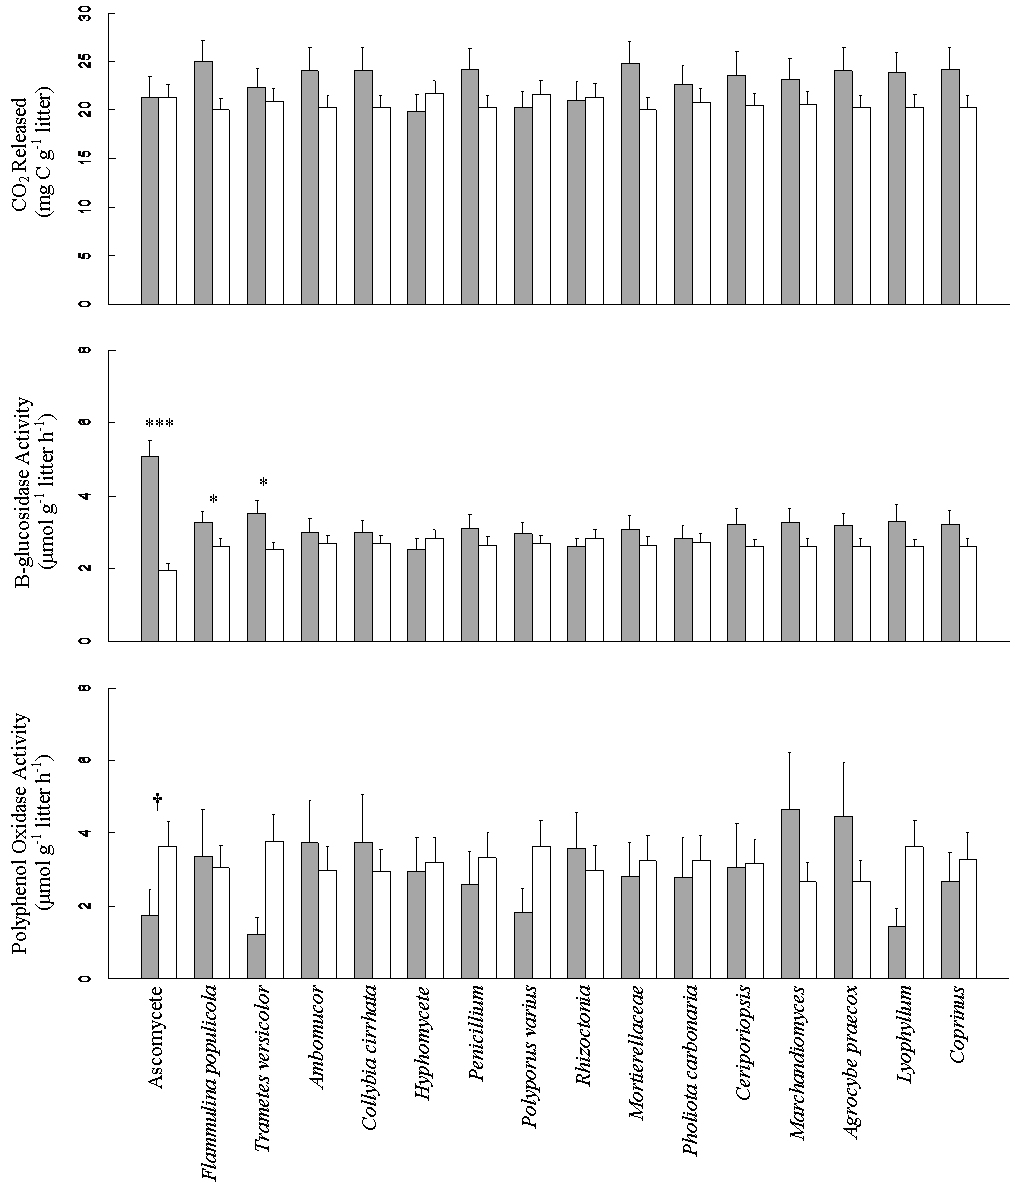
\includegraphics[width=5in]{obsbgppo.png}
\caption{The effect of presence (gray bars) and absence (hollow bars) of each species on decomposition (top), polyphenol oxidase (PPO) activity (middle) and $\beta$-glucosidase activity.  *** $P<0.0001$, * $P < 0.05$, $^{\dag}$ $P = 0.051$}
\label{fig:sp.presence.absence}
\end{figure}
%
\begin{figure}[p]
\centering 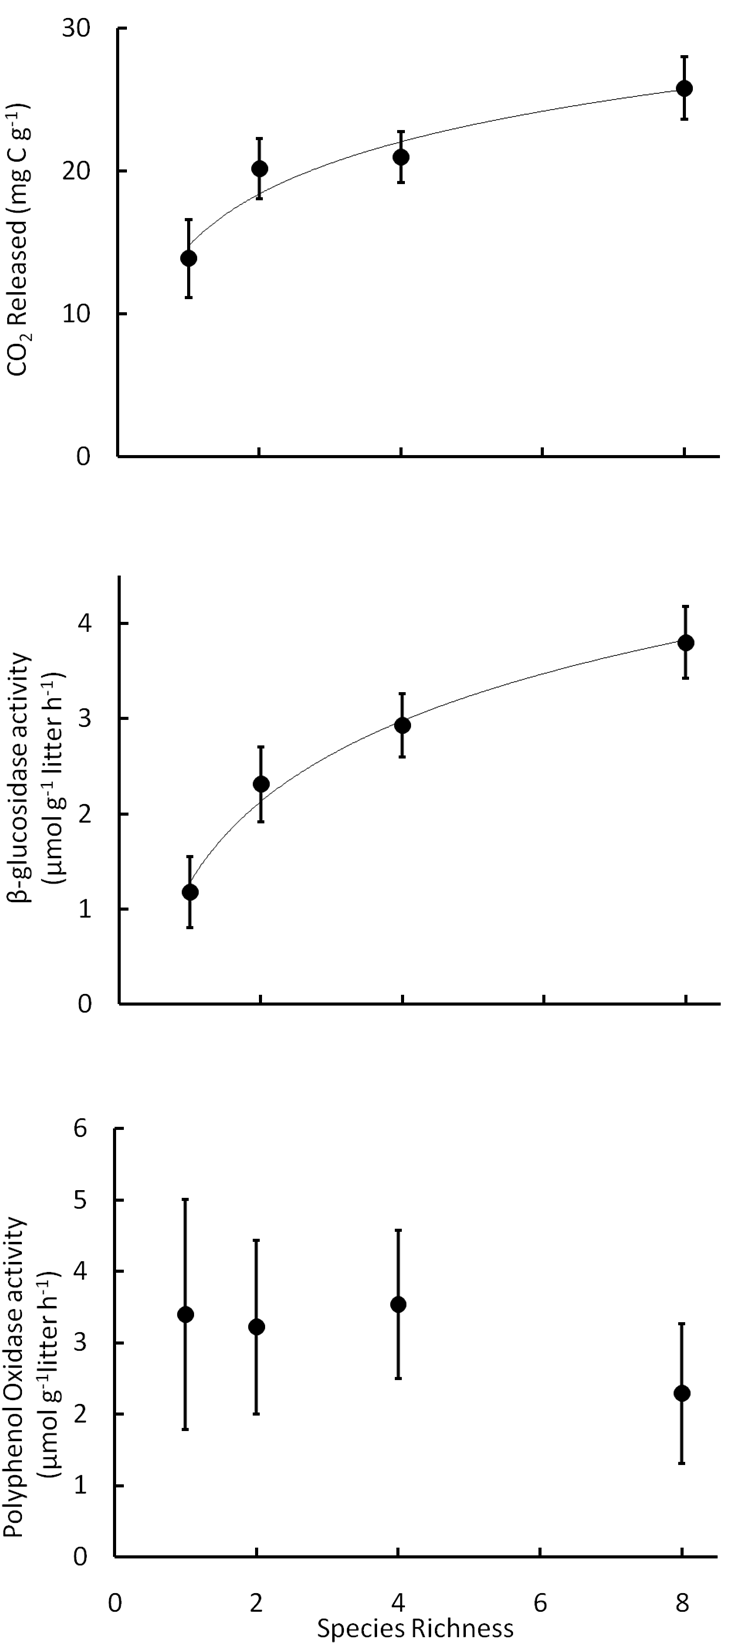
\includegraphics[width=4in]{obsbgppovspdiv.png} 
\caption{The effect of fungal species diversity on total decomposition (top, $P=0.03$), $\beta$-glucosidase activity (middle, $P<0.0001$), and polyphenol oxidase activity (bottom $NS$). Error bars represent the standard error of the mean.}

\label{fig:obs.bg.v.spdiv} 
\end{figure}

\end{document}
